\section{Overview}

\subsection{Principales características}
\begin{frame}
  \frametitle{Principales características}
  \begin{itemize}
    \item Android corre sobre Linux (v3.10).
    
    \item Android se aprovecha de Linux para:
      \begin{itemize}
	\item Abstracción de hardware.
	\item Administración de memoria.
	\item Administración de CPU.
	\item Networking.
	\item Seguridad.
      \end{itemize}
    
    \item El usuario no nota el Linux subyacente.
  \end{itemize}
\end{frame}

\subsection{Eimología e Historia}
\begin{frame}
  \frametitle{Eimología e Historia}
  \begin{itemize}
    \item Philip K. Dick
    \begin{figure}
	
\includegraphics[scale=0.1]{images/andy.png}
	\caption{Andy}
    \end{figure}
    
    \item Android Inc. $\rightarrow$ 2003.
    
    \item Google $\rightarrow$ 2005.
    
    \item OHA (Open Handset Alliance) $\rightarrow$ 2007.
    
    \item Primer version estable (v1.0) $\rightarrow$ 2008.
  \end{itemize}
\end{frame}

\subsection{Versionado}
\begin{frame}
  \frametitle{Versionado}
  \begin{itemize}
    \item Diversas versiones.    
    
    \item Nombre de dulces.
    
    \item Reparación de bugs y agregación de funciones.    
    
    \item v3.0 (Honeycomb), v4.0 (Ice Cream Sandwich), v5.1 (Lollipop).
  \end{itemize}
\end{frame}

\subsection{Stack}
\begin{frame}
  \frametitle{Stack}
  \begin{figure}
      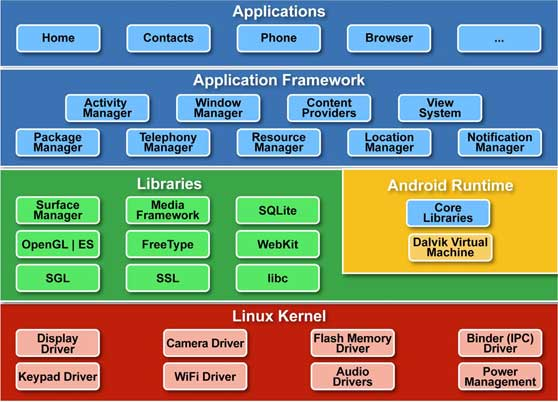
\includegraphics[scale=0.4]{images/stack.jpg}
  \end{figure}
\end{frame}

\subsection{Procesos e Hilos}
\begin{frame}
  \frametitle{Procesos e Hilos - Componentes}
  \begin{itemize}
    \item Cuando se invoca el primer componente de una aplicación se crea un proceso Linux con un único thread (\textit{main}/\textit{UI} thread).
    
    \item Por defecto todos los componentes de una aplicación se ejecutan sobre ese mismo thread.
    
    \item Los componentes pueden ser configurados para que ejecuten sobre diferentes procesos (\textit{android:process}).
    
    \item Es posible crear threads dentro de cada proceso $\rightarrow$ importante para el acceso a la \textit{UI}.
  \end{itemize}
\end{frame}

\begin{frame}
  \frametitle{Procesos e Hilos - Clasificación}
  \begin{itemize}
    \item Android elimina procesos bajo demanda ante la ausencia de memoria.
    
    \item Decición en base a Jerarquía de procesos clasificados en:
    \begin{itemize}
     \item \textit{Foreground process}
     \item \textit{Visible process}
     \item \textit{Service process}
     \item \textit{Background process}
     \item \textit{Empty process}
    \end{itemize}       
  \end{itemize}
\end{frame}

\begin{frame}
  \frametitle{Procesos e Hilos - Clasificación (cont.)}
  \begin{figure}
      \centering
      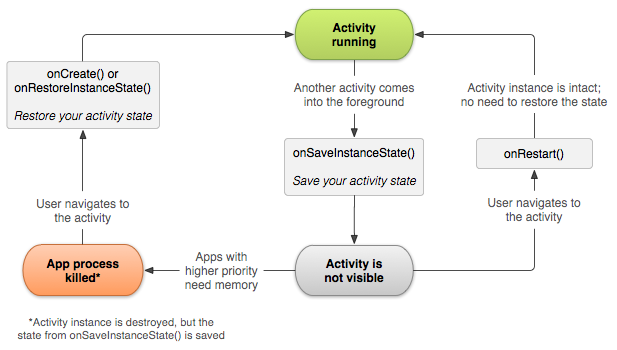
\includegraphics[scale=0.5]{images/restore-instance.png}
  \end{figure}
\end{frame}

\begin{frame}
  \frametitle{Procesos e Hilos - Dalvik Virtual Machine}
  \begin{itemize}
      \item Individualizada por cada aplicación.
      
      \item Cada proceso es un proceso Linux.
      
      \item Cada thread es un thread Linux.
      
      \begin{figure}
	\centering
	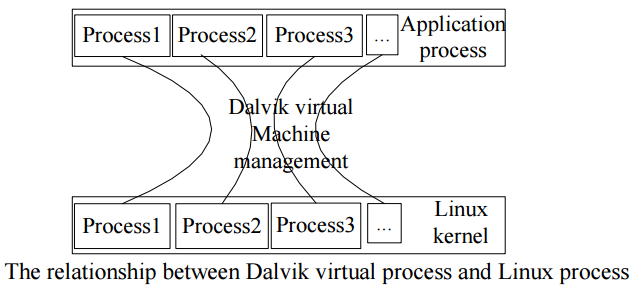
\includegraphics[scale=0.3]{images/dvm-linux-processes.png}
      \end{figure}
  \end{itemize}
\end{frame}

\subsection{DVM vs. JVM}
\begin{frame}
  \frametitle{DVM vs. JVM}  
  \begin{table}
      \centering
      \resizebox{\textwidth}{!}{
	  \begin{tabular}{| c | c |}
	      \hline
	      \bf DVM & \bf JVM \\
	      \hline
	      Máquina basada en registros & Máquina basada en stack \\
	      \hline
	      Diseñada para ejecutar sobre poca memoria & Consume más memoria \\
	      \hline
	      Ejecuta sus propios bytes codes (\textit{.dex}) $\rightarrow$ contiene multiples \textit{.class} & Ejecuta bytes codes Java (\textit{.class}) \\
	      \hline 
	      Uni-plataforma $\rightarrow$ Android & Multi-plataforma \\
	      \hline
	      Ejecutable $\rightarrow$ \textit{.apk} & Ejecutable $\rightarrow$ \textit{.jar} \\
	      \hline
	  \end{tabular}
      }
  \end{table}
\end{frame}

\subsection{Aplicaciones}
\begin{frame}
  \frametitle{Aplicaciones - Building}
  \begin{itemize}
    \item Un \textit{android package} contiene todo lo necesario para ejecutar la aplicación en un dispositivo.
    
    \item \textbf{Gradle} es el \textit{application builder} oficial del \textit{SDK} de Android (\textit{gradle.build}).
    \begin{itemize}
	\item Debug mode $\rightarrow$ automático.
	\item Release mode.
    \end{itemize}
  \end{itemize}
  
  \begin{figure}
    \centering
    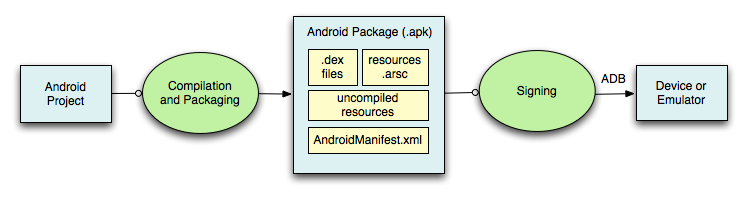
\includegraphics[scale=0.4]{images/build-app.png}
  \end{figure} 
\end{frame}

\begin{frame}
  \frametitle{Aplicaciones - Launching}
    \begin{figure}
      \centering
      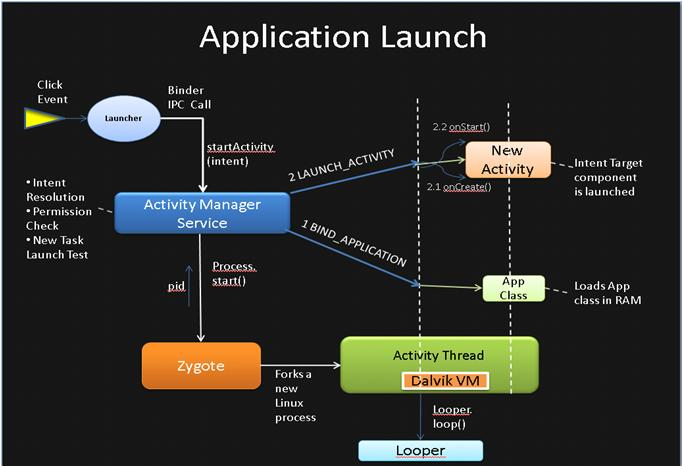
\includegraphics[scale=0.5]{images/launch-app.jpg}
    \end{figure}
\end{frame}

\subsection{Seguridad}
\begin{frame}
  \frametitle{Seguridad - Datos de aplicación}
  \begin{itemize}
    \item Ninguna aplicación puede ejecutar operaciones que afecten a las demás.
    
    \item Solo pueden escribir y leer datos privados de la aplicación.
    
    \item Las aplicaciones comparten datos de manera explícita.    
  \end{itemize}
\end{frame}

\begin{frame}
  \frametitle{Seguridad - Id. de usuario y permisos sobre archivos}
  \begin{itemize}
    \item Cuando se instala un \textit{.apk}, Android le otorga un \textit{userId} de Linux definitivo.
    
    \item En otro dispositivo el mismo paquete podría tener otro \textit{userId}.
    
    \item Dos aplicaciones con el mismo \textit{userId} son tratadas como la misma aplicación.
    
    \item Mismo \textit{userId} = Mismo usuario Linux = Misma aplicación = Mismos permisos sobre los archivos de la aplicación.
    
    \item Las aplicaciones que comparten el \textit{userId} tienen que compartir la firma. Es decir que deben ser firmados por la misma clave privada.        
  \end{itemize}
\end{frame}

\begin{frame}
  \frametitle{Seguridad - Ejemplo shared user id}
  \begin{figure}
    \centering
    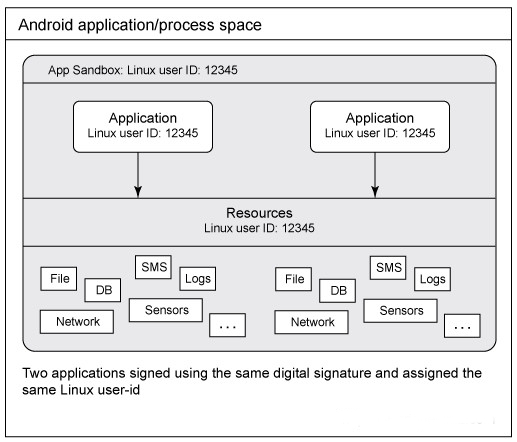
\includegraphics[scale=0.4]{images/two-same-apps.jpg}
  \end{figure}
\end{frame}

\begin{frame}[fragile]
  \frametitle{Seguridad - Recursos}
  \begin{itemize}
    \item Se debe declarar el acceso a los recursos de manera estática (\textit{Manifest.xml}).
    
    \item Cuando la aplicación es instalada el usuario debe dar su consentimiento.
    
    \item \textit{SecurityException}
    \begin{lstlisting}
<manifest xmlns:android="http://schemas.android.com/apk/res/android"
    package="com.android.app.myapp" >

    <uses-permission android:name="android.permission.RECEIVE_SMS" />
    ...
</manifest>
    \end{lstlisting}    
  \end{itemize}
\end{frame}

\begin{frame}
  \frametitle{Seguridad - Application sandbox}
  \begin{figure}
    \centering
    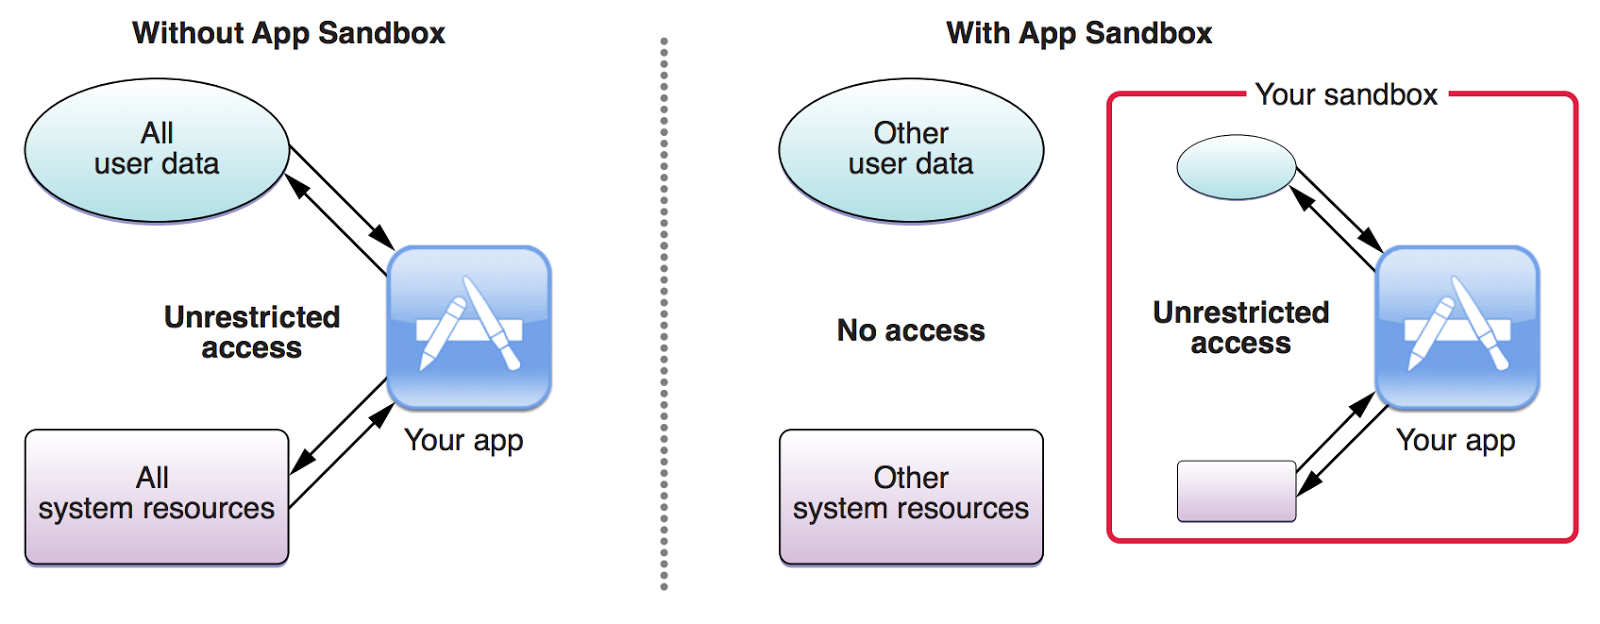
\includegraphics[scale=0.2]{images/sandbox.png}
  \end{figure}
  
  \begin{itemize}
      \item Solo una porción de código Android corre como \textit{root}.
      
      \item ¿Cómo hacen diferentes reproductores para acceder a la música?
  \end{itemize}
\end{frame}

\begin{frame}
  \frametitle{Seguridad - Signing}
  \begin{itemize}
    \item Todas las aplicaciones (\textit{.apk}) tienen que ser firmados digitalmente.

    \item Se emiten certificados auto-firmados (\textit{KeyTool}):
    \begin{itemize}
	\item Debug mode $\rightarrow$ \textit{debug key} $\rightarrow$ el \textit{keystore} se crea automáticamente (\textit{\$HOME/.android}).
	
	\item Release mode $\rightarrow$ \textit{developer's private key} $\rightarrow$ manualmente.
    \end{itemize}    
  \end{itemize}
\end{frame}

\begin{frame}
  \frametitle{Seguridad - Repaso y Overview}
  \begin{itemize}
   \item A nivel de \textit{AndroidManifest} $\rightarrow$ permisos a recursos que termina de conseder el usuario (aplicado por el \textit{sandbox}).
   
   \item A nivel de las aplicaciones y sus archivos $\rightarrow$ certificado, \textit{userId} y permisos \textit{UGO} (aplicado por el \textit{sandbox}).
   
   \item A nivel de file system $\rightarrow$ particiones \textit{read-only} (/system).   
  \end{itemize}
\end{frame}

\subsection{Almacenamiento}
\begin{frame}
  \frametitle{Almacenamiento}
  \begin{itemize}
      \item SQLite: 
      \begin{itemize}
	  \item Se maneja a través de una biblioteca.
	  
	  \item Bajo licencia \textit{GPL}.
	  
	  \item Actúa sobre archivos ordinarios.

	  \item Cumple las propiedades ACID.
	  
	  \item \textit{/data/data/$<$package\_name$>$/databases/}
      \end{itemize}
      
      \item Shared preferences
      \begin{itemize}
	  \item Se puede manejar una colección de ellas.
	  
	  \item Se almacenan a través de archivos XML.
	  
	  \item Se identifican a través del nombre que se le da al archivo.
	  
	  \item Pueden ser privadas (\textit{MODE\_PRIVATE}) o compartidas (\textit{MODE\_WORLD\_READABLE} o \textit{MODE\_WORLD\_WRITEABLE}).
	  
	  \item \textit{/data/data/$<$package\_name$>$/shared\_prefs/}
      \end{itemize}
  \end{itemize}
\end{frame}

\subsection{File System}
\begin{frame}[fragile]
  \frametitle{File system - Tipos de memorias}
  \begin{itemize}
      \item Raw NAND flash:
      \begin{itemize}
	  \item Subsistema \textit{MTD}.
	  
	  \item \textit{/dev/block/mtdblockN}
	  
	  \begin{lstlisting}
$ cat /proc/mtd                                                 
dev:    size   erasesize  name
mtd0: 05660000 00020000 "system"
mtd1: 04000000 00020000 "userdata"
mtd2: 04000000 00020000 "cache"
	  \end{lstlisting}
      \end{itemize} 
      
      \item SD, MicroSD y eMMC:
      \begin{itemize}
	  \item Driver \textit{mmcblock}.
	  
	  \item \textit{/dev/block/mmcblk[chip number]p[partition number]}
	  
	  \begin{lstlisting}
$ ls -l /dev/block/platform/msm_sdcc.1/by-name
cache -> /dev/block/mmcblk0p36
system -> /dev/block/mmcblk0p38
userdata -> /dev/block/mmcblk0p40
	  \end{lstlisting}
      \end{itemize}
  \end{itemize}
\end{frame}

\begin{frame}
  \frametitle{File system - Tipos}
  \begin{itemize}
      \item YAFFS
      \begin{itemize}
	\item Booteo más rápido.
	
	\item Consume menos memoria.
	
	\item Divide los archivos en páginas.
	
	\item \textit{GPL}.
	
	\item v1 y v2.
	
	\item Single-theading.
	
	\item Hasta \textbf{Froyo} (v2.2).
	
	\item Especializado para funcionar en memorias de tipo raw NAND.
      \end{itemize}
      
      \item Ext4
      \begin{itemize}
	\item Multi-theading.
	
	\item Desde \textbf{Gingerbread} (v2.3).
	
	\item Utilizado generalmente en memorias SD, MicroSD o eMMC.
      \end{itemize}   
  \end{itemize}
\end{frame}

\begin{frame}[fragile]
  \frametitle{File system - Puntos de montaje principales}
  \begin{itemize}
      \item \textit{/system}
      
      \item \textit{/system/bin}
      
      \item \textit{/data/app}
      
      \item \textit{/data/data/$<$package\_identifier$>$}
      
      \item \textit{/recovery}
      
      \item \textit{/boot}
      
      \item \textit{/cache}
  \end{itemize}
\end{frame}

\subsection{Licencia}
\begin{frame}
  \frametitle{Licencia}
  \begin{itemize}
      \item La idea de \textbf{Google} es mantener \textit{GPL} fuera del espacio de usuario:
      \begin{itemize}
	  \item \textit{Apache v2} para el espacio de usuario.
	  
	  \item \textit{GPL} para el espacio de kernel.
      \end{itemize}
      
      \item Además de tamaño y optimización, esta fue otra de las razones por las que implementaron su propia version de \textit{libc} (\textit{BIONIC}).
  \end{itemize}
\end{frame}